\documentclass[11pt,a5paper]{article}

\usepackage[T1]{fontenc}
\usepackage[utf8]{inputenc}
\usepackage{lmodern, microtype}
\usepackage[estonian]{babel}
\usepackage{siunitx}
\sisetup{inter-unit-product=\ensuremath{{}\cdot{}}, per-mode=fraction, exponent-product=\cdot, output-decimal-marker={,}, uncertainty-mode=separate}
\usepackage{graphicx}
\usepackage{wrapfig}
\usepackage{tikz}
\usetikzlibrary{arrows.meta, patterns, patterns.meta}
\usepackage[european]{circuitikz}
\usepackage{pgfplots}
\tikzset{component/.style={draw,thick,circle,fill=white,minimum size=0.75cm,inner sep=0pt}}
\usepackage{amsmath,amssymb,amsfonts}
\usepackage[hidelinks]{hyperref}
\usepackage{csquotes}
\usepackage{caption}
\usepackage{enumitem}
\topmargin=-3.0cm \textheight=19cm \textwidth=12.9cm
\oddsidemargin=-1.5cm  \evensidemargin=-1.5cm
\setlength{\parindent}{0pt} \setlength{\parskip}{6pt} \sloppy
\sloppy \relpenalty=10000 \binoppenalty=10000
\pagestyle{empty}


\newcommand{\numb}[1]{\vspace{5pt}\textbf{\large #1}}
\newcommand{\nimi}[1]{(\textsl{\small #1})}
\newcommand{\punktid}[1]{(\emph{#1~p.})}
\newcommand{\p}[1]{[\textbf{#1~p}]}
\newcounter{ylesanne}
\newcommand{\yl}[1]{\addtocounter{ylesanne}{1}\numb{\theylesanne.} \nimi{#1} \newblock{}}
%\newcommand{\autor}[1]{}% Kasuta võistluse ajal
\newcommand{\autor}[1]{\emph{Autor: #1}}% Kasuta kui vaja autorit
\newcommand{\autorl}[1]{\emph{Lahenduse autor: #1}}% Kasuta kui vaja autorit



\pgfplotsset{compat=1.18}
\begin{document}
\normalsize
\begin{center}
  \textbf{\Large Eesti koolinoorte 69.\ füüsikaolümpiaad} \par
  \emph{9.\ aprill 2022. a.\\ \textbf{Gümnaasiumi} ülesannete lahendused (10.--12.\ klass)}
\end{center}

\normalsize

\yl{KETTAHEIDE}
\punktid{6} \autor{Jaan Kalda}\\

\begin{figure}[h]
    \centering
    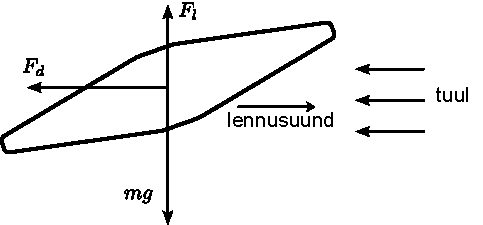
\includegraphics[]{ketas-lah.pdf}
\end{figure}

Jõudiagramm on toodud joonisel. Vastutuul suurendab nii takistusjõudu kui õhuvoolust tingitud üleslükkejõudu. Üleslükkejõud kasvab proportsionaalselt ketta kiirusega õhu suhtes. Suurem üleslükkejõud pikendab lennuaega, mille tulemusel jõuab ketas liikuda horisontaalsihis kaugemale vaatamata sellele, et horisontaalsuunaline kiirus natuke väheneb takistusjõu tõttu (esimene efekt on tugevam, kui teine).

\yl{LUMEVÄLI}
\punktid{8} \autor{Moorits Mihkel Muru}\\
Olgu väljaku pikem külg \(a\), lühem külg \(b\), Mari kiirus mööda teed \(v\) ja kiirus läbi lume \(nv\). Mari keerab tee pealt lumisele väljakule hetkel, kui tal oli veel jäänud mööda teed platsi nurgani liikuda \(x\) meetrit ning liigub üle väljaku otse läbi lume koolimaja ukse suunas. Sellisel juhul liigub Mari mööda pikemat külge teepikkuse \(s_1 = a - x\) ja pärast seda diagonaalis \(s_2 = \sqrt{x^2 + b^2}\). Mööda väljaku äärt liikudes kuluks Maril ukseni jõudmiseks
\[
    t_0 = \frac{a + b}{v}
\]
ja üle väljaku joostes kulub ukseni jõudmiseks
\[
    t_1 = \frac{s_1}{v} + \frac{s_2}{nv} = \frac{a}{v} - \frac{x}{v} + \frac{\sqrt{x^2 + b^2}}{nv} \ .
\]
Selleks, et leida, millise nurga all peaks Mari läbi lume jooksma, saame kasutada optikast tuttavat murdumisseadust
\[
    \frac{\sin \alpha}{\sin \gamma} = \frac{v}{nv} \ ,
\]
kus keskkondasid lahutav sirge on väljaku serv ning seega \(\alpha = \ang{90}\), sest Mari liikus kõigepealt mööda väljaku serva, ning \(\gamma\) on nurk väljaku serva ristsirge ning Mari optimaalse liikumissuuna vahel. Seega \(\sin \alpha = 1\) ja saame
\[
    \sin \gamma = \frac{nv}{v} = n
\]
ning geomeetriast saame
\[
    \sin \gamma = \frac{x}{s_2} \quad \Rightarrow \quad \frac{x}{s_2} = n \quad \Rightarrow \quad x = n s_2 = n \sqrt{x^2 + b^2} \ .
\]
Avaldame saadud võrrandist \(x\)-i.
\begin{align*}
    x &= n \sqrt{x^2 + b^2} \ , \\
    x^2 &= n^2 (x^2 + b^2) \ , \\
    x^2 - n^2 x^2 &= n^2 b^2 \ , \\
    x^2 &= \frac{n^2 b^2}{1 - n^2} \ , \\
    x &= \frac{n b}{\sqrt{1 - n^2}} \ .
\end{align*}
Asendame leitud \(x\)-i väärtuse \(t_1\) avaldisse.
\[
    t_1 = \frac{a}{v} - \frac{n b}{v\sqrt{1 - n^2}} + \frac{\sqrt{\left(\frac{n b}{\sqrt{1 - n^2}}\right)^2 + b^2}}{n v} = \frac{a}{v} - \frac{b}{v} \frac{n}{\sqrt{1-n^2}} + \frac{\sqrt{\frac{n^2 b^2}{1 - n^2} + b^2}}{n v} = 
\]
\[
    = \frac{a}{v} - \frac{b}{v} \frac{n}{\sqrt{1-n^2}} + \frac{b}{v} \frac{\sqrt{\frac{n^2 + 1 - n^2}{1-n^2}}}{n} = \frac{a}{v} - \frac{b}{v} \frac{n}{\sqrt{1-n^2}} + \frac{b}{v} \frac{1}{n\sqrt{1-n^2}} \ .
\]
Leiame aegade erinevuse üle ja ümber väljaku liikudes.
\begin{align*}
    \Delta_t = t_0 - t_1 &= \frac{a}{v} + \frac{b}{v} - \left( \frac{a}{v} - \frac{b}{v} \frac{n}{\sqrt{1-n^2}} + \frac{b}{v} \frac{1}{n\sqrt{1-n^2}} \right) = \\
    &= \frac{b}{v} \left( 1 + \frac{n}{\sqrt{1-n^2}} - \frac{1}{n\sqrt{1-n^2}} \right) \ .
\end{align*}
Leiame ajavõidu kasutades ülesande tekstis antud suuruseid.
\[
    \Delta_t = \frac{\SI{50}{\metre}}{\SI{6}{\metre\per\second}} \left( 1 + \frac{\num{0.8}}{\sqrt{1-\num{0.8}^2}} - \frac{1}{\num{0.8}\sqrt{1-\num{0.8}^2}} \right) \approx \SI{2.1}{\second} \ .
\]
Seega oleme näidanud, et ümber väljaku liikumine on \(\Delta_t \approx \SI{2.1}{\second}\) võrra aeglasem kui üle väljaku mööda optimaalset trajektoori. \\

Alternatiivselt saab leida \(x\)-i väärtuse ka ilma murdumisseaduseta lahendades ekstreemum ülesande, et leida \(x\)-i väärtust, mis minimeerib \(t_1\) avaldist.
\[
    t_1'(x) = 0 - \frac{1}{v} + \frac{1}{2} \frac{2x}{nv\sqrt{x^2 + b^2}} = \frac{x}{nv\sqrt{x^2 + b^2}} - \frac{1}{v} = 0 \ .
\]
Lahendame saadud võrrandi.
\begin{align*}
    \frac{x}{nv\sqrt{x^2 + b^2}} &= \frac{1}{v} \ , \\
    x &= \frac{nv\sqrt{x^2 + b^2}}{v} \ , \\
    x^2 &= n^2 (x^2 + b^2) \ , \\
    x^2 - n^2 x^2 &= n^2 b^2 \ , \\
    x^2 &= \frac{n^2 b^2}{1 - n^2} \ , \\
    x &= \frac{nb}{\sqrt{1 - n^2}} \ .
\end{align*}
Näeme, et tulemus on sama, mis murdumisseadusest.



\yl{SILINDER}
\punktid{8} \autor{Richard Luhtaru}\\
Jagame silindri kaheks poolsilindriks. Me võime vaadelda kumbagi poolsilindrit kui hästi laia juhet, mille pikkus on $\ell = \pi r$ ja ristlõikepindala on $S = \tau h$. Kummagi poolsilindri takistus on seega
\begin{equation*}
    R = \rho \frac{\ell}{S} = \frac{\rho \pi r}{\tau h}
\end{equation*}

Kuna kaks ``juhet'' on ühendatud rööbiti, siis kogutakistus A ja B vahel on
\begin{equation*}
    R_{AB} = \frac{1}{2}R = \frac{\rho \pi r}{2\tau h}
\end{equation*}

\newpage
\yl{LÄÄTSEDE KOLMNURK}
\punktid{8} \autor{Erkki Tempel}\\

\begin{figure}[h]
    \centering
    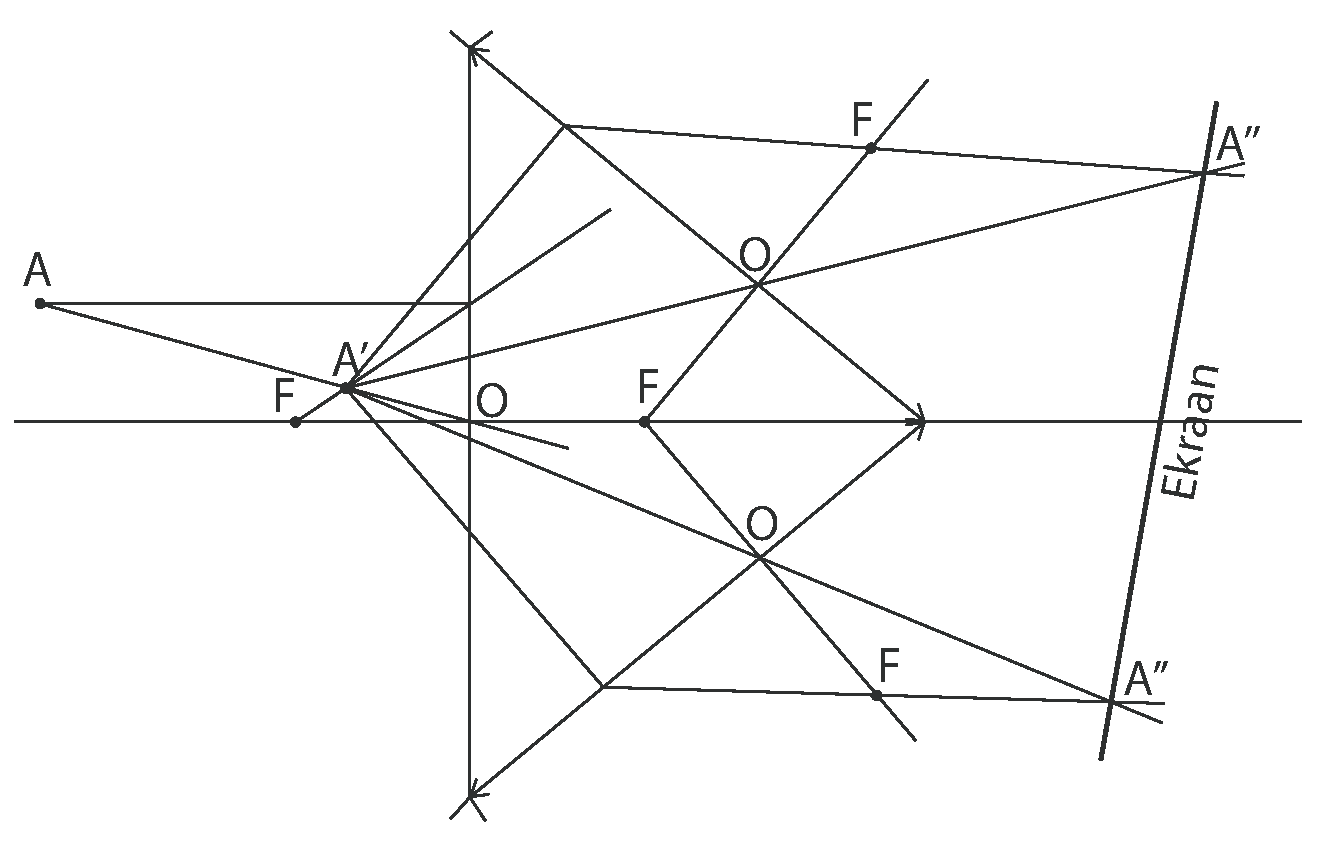
\includegraphics[scale=0.5]{joonislah.pdf}
\end{figure}

\yl{JALGRATAS} \punktid{8} \autor{Valter Kiisk}\\
\osa Olgu otsitav tõusunurk $\alpha$. Raskusjõu komponent, mis on suunatud piki mäenõlva alla, on siis $F=mg\sin\alpha$. Piirjuhul mõjub sama jõuga ka maapind ratastele. Seega saame tingimuse $Fr=M$, millest avaldame nurga
\[
\alpha=\arcsin\left( \frac{M}{mgr}\right)\approx \SI{9.7}{\degree}.
\]

\osa Liikugu jalgratas mäest üles kiirusega $v$. Jalgratta masskese tõuseb seega kiirusega $v\sin\alpha$ ja potentsiaalne energia kasvab vastavalt tempoga $mgv\sin\alpha$. Kui muid energiakadusid ei ole, siis see peab olema võrdne mootori kasuliku võimsusega $P$. Sellest saame avaldada kiiruse
\[
v=\frac{P}{mg\sin\alpha}\approx \SI{5.3}{\meter\per\second}.
\]

\textit{Märkus:} oluline tähelepanek on asjaolu, et maksimaalse tõusunurga puhul on piiravaks teguriks mootori pöördemoment ning tõusunurk ei sõltu mootori võimsusest. See tuleneb sellest, vaatleme liikuma hakkamist tühiselt väikesel kiirusel. Maksimaalse kiiruse puhul on aga piiravaks teguriks võimsus, kuna etteantud kaldenurk on väiksem maksimaalsest võimalikust kaldenurgast.


\yl{ÕHUPÜSS} \punktid{10} \autor{Jaan Kalda} \\
Torus toimub gaasi adiabaatiline paisumine, kusjuures sõltumata toru pikkusest omandab gaas torus pärast kuuli välja lendamist toas valitseva õhurõhu. Seega on jäävad suurused nii $pV^\gamma$ kui $pV/T$, millest saame, et jääv suurus on ka $p^{\gamma-1}/T^\gamma$. Siit saame juba avaldada küsitud temperatuuri:
$$
T_1=T_0(p_0/p_1)^{\frac{\gamma - 1}{\gamma}}=T_0(p_0/p_1)^{2/7} \approx \SI{55}{\kelvin} \approx \SI{-218}{\celsius}
$$
\textit{Märkus:} tulemus on väiksem lämmastiku keemistemperatuurist, seega tegelikult langeb lämmastiku temperatuur keemistemperatuurini $\SI{-196}{\celsius}$ ning edasise paisumise juures püsib see konstantsena tänu vabanevale aurustumissoojusele.
\textit{PS:} adiabaadinäitaja on ka leitav valemiga $\gamma=c_P/c_V=(c_V+R)/c_V=1.4$.

\yl{VEEUPUTUS} \punktid{10} \autor{Oleg Ko\v sik}\\
Paneme tähele, et \SI{1}{l\per m^2}=\SI{1}{mm} ehk otsitav torustiku äravool on arvuliselt võrdne äraveetavate sademete hulgaga millimeetrites.

Olgu $h_6=\SI{22}{\mm}$ sademete koguhulk 6 minuti järel ning $h_9=\SI{28}{\mm}$ omakorda 9 minuti järel, $H$ mitu millimeetrit sademeid suudab endas mahutada kraav (kui äravoolu ei oleks) ning $u$ töökorras torustiku sademete äravoolu kiirus millimeetrites minutis.

Saame võrrandid
\[
h_6 = H +0.5 u \cdot \SI{6}{\min}
\]
ja
\[
h_9 = H + u \cdot \SI{9}{\min}
\]
Sellest võrrandisüsteemist leiame $H=\SI{19}{\mm}$.

Olgu otsitud äravoolu kiirus $u_x$. Siis sirge $h(t)=H+u_xt$ näitab, kui palju suudab kanalisatsioonisüsteem akumuleerida vett maksimaalselt igal ajahetkel ($H$ on kraavi panus $u_xt$ sadeveetorustiku panus). Selleks, et uputus ei tekiks, peab sademete koguhulga graafik jääma alati sellest sirgest allapoole. Kiirus $u_x$ on minimaalne siis, kui see sirge on graafiku puutuja. Tõmbame niisiis graafikult puutuja, mis läbib punkti $(0,H)$. Selle puutuja tõus on otsitav kiirus $u_x$. Mõõtmised annavad meile $u_x=\SI{1.23}{mm/min}=\SI{1.23}{\L\per\m\squared}$ minutis.

\begin{figure}[h]
	\vspace{-1em}
    \centering
    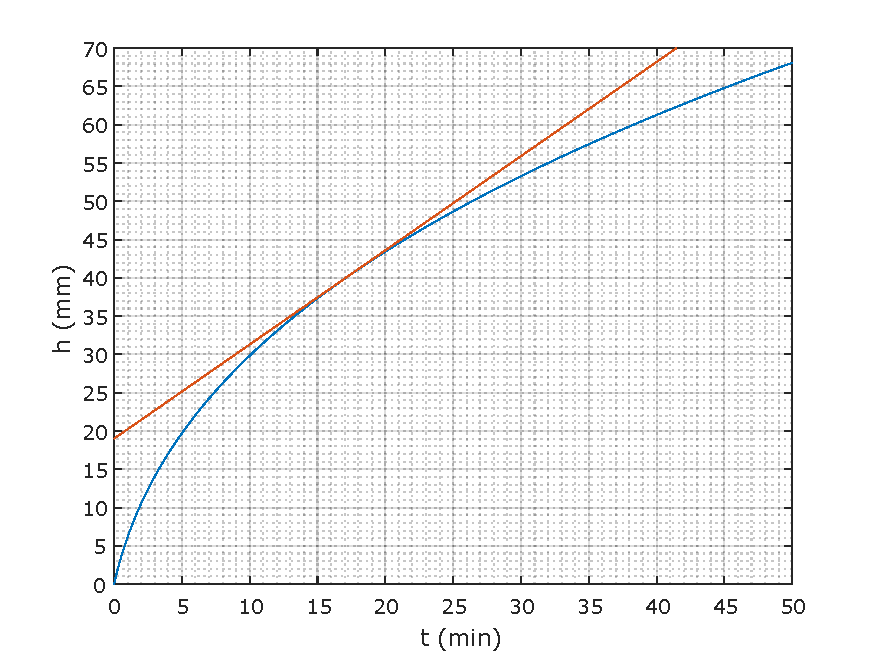
\includegraphics[width=0.75\linewidth]{uputus_lah.pdf}
\end{figure}

\newpage
\yl{VEEVALAJA} \punktid{12} \autor{Kaur Aare Saar}\\
Arvestama peab kolme efektiga:
\begin{itemize}
\item Ülemise anuma mass muutub väiksemaks kiirusega $\dot{m}$. See toimub esimese $\frac{m}{\dot{m}}=\SI{1}{\second}$ jooksul.
\item Alumise anuma mass muutub suuremaks kiirusega $\dot{m}$. See algab ajahetkel $t_1=\sqrt{\frac{2h}{g}}= \SI{0.45}{\second}$ ja kestab kuni hetkeni $t_2 = t_1 + \frac{m}{\dot{m}} = \SI{1.45}{\second}$.
\item Kui vesi jõuab alumisse anumasse, siis avaldab ta läbi Olegi kaalule jõudu mis on võrdne anumasse jõudva impulsi muutumise kiirusega, s.o. $F = \frac{\Delta (mv)}{\Delta{t}} = \dot{m}v = \dot{m} \sqrt{2gh}$, mis mõjub konstatselt vahemikus $t_1$ kuni $t_2$. See vastab kaalu näidu muutusega $m_p = \frac{\dot{m} \sqrt{2gh}}{g} = \dot{m}\sqrt{\frac{2h}{g}}= \SI{0.45}{\kilo\gram}$
\end{itemize}
Need kolm komponenti kokku liites saame järgneva graafiku:

\begin{figure}[h]
\centering
  \begin{tikzpicture}
    \begin{axis}[
      xmin=0, xmax=1.5,
      ymin=-1, ymax=1,
      xlabel=$t$ (s),
      ylabel=$m$ (kg),
    ]
      \addplot[]
      coordinates{
        (0,0)
        (0.45,-0.45)
        (0.45,0)
        (1,0)
        (1.45,0.45)
        (1.45,0)
        (1.5,0)
      };
    \end{axis}
  \end{tikzpicture}
\end{figure}

\yl{SATELLIIT} \punktid{12} \autor{Jaan Kalda} \\
Kui satelliit oleks kahe absoluutselt musta plaadi vahel, mille temperatuur on $T_0$, siis saavutaks ta peatselt soojusliku tasakaalu, st omandaks temperatuuri $T_0$. Sellisel juhul kiirgaks ta soojust koguvõimsusega $P_0=S \sigma T^4_0$, kus $S$ on ta kogupindala. Nüüd saab ta aga soojuskiirgust kaks korda vähem seetõttu, et on vaid üks plaat. Arvestades Maa ja musta plaadi soojuskiirguste tiheduste suhtega $\epsilon$, saame satelliidile langeva koguvõimsuse $P_1=\epsilon S \sigma T^4_0/2$. Soojustasakaalu korral kiirgab satelliit sama palju, kui ta saab soojust, st $\epsilon S \sigma T^4_0/2=S \sigma T^4$. Siit saame avaldada satelliidi temperatuuri:
$$
T=(\epsilon/2)^{1/4}T_0 \approx \SI{213}{\kelvin} \approx \SI{-60}{\celsius}. 
$$

\yl{PLAAT} \punktid{12} \autor{Konstantin Dukats}\\
Kui metallist plaat viiakse laengu elektrivälja, indutseerub selle peal laeng nii, et see kompenseerib välise elekrivälja (st plaadi sees paigutuvad laengud vastavalt ümber, kuni elektrivälja tugevus plaadis on null). Kuna $r \ll R$, saame eeldada, et laengute pindtihedused on mõlemal küljel on isotroopsed. Kuna plaadi kogulaeng on null, siis indutseeritud laeng plaadi pindadel on vastavalt $\pm \Delta q$. Plaat sarnaneb sellel juhul laetud kondensaatoriga. Kuna plaadi sees on elektrivälja tugevus null, siis peab välise elektrvälja ja indutseeritud elektrivälja summa olema $0$ ehk $\vec{E}_q + \vec{E}_{\pm \Delta q}=0$. Siit saame avaldada ümberpaigutunud laengu suuruse $\Delta q$:

$$\therefore \frac{1}{4\pi \varepsilon_0} \frac{q}{R^2} = \frac{\Delta q}{2 \pi r^2} - \frac{-\Delta q}{2 \pi r^2},$$
$$\frac{1}{4\pi \varepsilon_0} \frac{q}{R^2} = \frac{\Delta q}{\pi r^2},$$
\begin{equation}
\Delta q = \frac{1}{4\pi \varepsilon_0} \frac{q}{R^2} \pi r^2.
\end{equation}
Coulomb'i seadusest avaldame jõu, mis rakendub vastavalt kummalegi plaadi pinnale ning saame summarseks jõuks:
\begin{equation}
F = \frac{1}{4 \pi \varepsilon_0} \frac{q \Delta q}{R^2} - \frac{1}{4 \pi \varepsilon_0} \frac{q \Delta q}{(R+h)^2} \approx \frac{q \Delta q}{4 \pi \varepsilon_0} \frac{2Rh}{R^4},
\end{equation}
Võrranditest (1) ja (2) saame asendades:
$$F \approx \frac{q^2 h r^2}{8 \pi \varepsilon_0 R^5}.$$



\end{document}